\subsection{线段和比较的度量}\label{subsec:czjh1-1-3}

在生产实践和日常生活中,经常需要比较线段的大小和度量线段的长度。
例如,比较两个人的高矮就是比较线段的大小的例子,量一个同学的身高就是度量线段长度的例子。

比较人的高矮时,两人要并立在平地上,才能比较出高矮来,
比较两条线段的大小(通常说长短),也是用类似的方法。

如图 \ref{fig:czjh1-1-12} ,把线段 $AB$ 放到线段 $A'B'$ 上,使点 $A$ 和点 $A'$ 重合,
$AB$ 沿着 $A'B'$ 的方向落下。那么有下面三种可能情形:

\begin{figure}[htbp]
    \centering
    \begin{minipage}[b]{4cm}
        \centering
        \begin{tikzpicture}
	\tkzDefPoints{0/0/A, 1.5/0/B}
	\tkzDrawSegment(A,B)
	\tkzDrawPoints[fill=black](A,B)
	\tkzLabelPoints[above](A,B)

	\tkzDefPoints{0/-1/A', 1.5/-1/B'}
	\tkzDrawSegment(A',B')
	\tkzDrawPoints[fill=black](A',B')
	\tkzLabelPoints[above](A',B')
	\tkzLabelPoint[below](A'){$(A)$}
	\tkzLabelPoint[below](B'){$(B)$}
\end{tikzpicture}


        \caption*{甲}
    \end{minipage}
    \qquad
    \begin{minipage}[b]{4cm}
        \centering
        \begin{tikzpicture}
	\tkzDefPoints{0/0/A, 1.5/0/B}
	\tkzDrawSegment(A,B)
	\tkzDrawPoints[fill=black](A,B)
	\tkzLabelPoints[above](A,B)

	\tkzDefPoints{0/-1/A', 1.5/-1/B, 2.0/-1/B'}
	\tkzDrawSegment(A',B')
	\tkzDrawPoints[fill=black](A',B',B)
	\tkzLabelPoints[above](A',B',B)
	\tkzLabelPoint[below](A'){$(A)$}
\end{tikzpicture}


        \caption*{乙}
    \end{minipage}
    \qquad
    \begin{minipage}[b]{4cm}
        \centering
        \begin{tikzpicture}
	\tkzDefPoints{0/0/A, 1.5/0/B}
	\tkzDrawSegment(A,B)
	\tkzDrawPoints[fill=black](A,B)
	\tkzLabelPoints[above](A,B)

	\tkzDefPoints{0/-1/A', 1.0/-1/B', 1.5/-1/B}
	\tkzDrawSegment(A',B)
	\tkzDrawPoints[fill=black](A',B',B)
	\tkzLabelPoints[above](A',B',B)
	\tkzLabelPoint[below](A'){$(A)$}
\end{tikzpicture}


        \caption*{丙}
    \end{minipage}
    \caption{}\label{fig:czjh1-1-12}
\end{figure}

(1) 如图 \ref{fig:czjh1-1-12} 甲, 点 $B$ 与 $B'$ 重合,这时两条线段相等,记作 $AB = A'B'$;

(2) 如图 \ref{fig:czjh1-1-12} 乙, 点 $B$ 落在线段 $A'B'$ 上($A'$、$B'$ 之间),
这时线段 $AB$ 小于线段 $A'B'$(或说线段 $A'B'$ 大于线段 $AB$),
记作 $AB < A'B'$ (或 $A'B' > AB$〉。

(3) 如图 \ref{fig:czjh1-1-12} 丙, 点 $B$ 落在线段 $A'B'$ 的延长线上,也就是点 $B'$ 在线段 $AB$ 上,
这时 $AB > A'B'$(或 $A'B' < AB$)。

在小学时,我们曾使用刻度尺来度量线段的长度。
以后,我们还可以象图 \ref{fig:czjh1-1-13} 那样,利用两脚规配合刻度尺来进行度量。
例如,在图 \ref{fig:czjh1-1-13} 中,量得线段 $AB$ 的长度是 $3.1 \; \limi$. 记作 $AB = 3.1 \; \limi$。

\begin{figure}[htbp]
    \centering
    \begin{minipage}[b]{7cm}
        \begin{minipage}[b]{3cm}
            \centering
            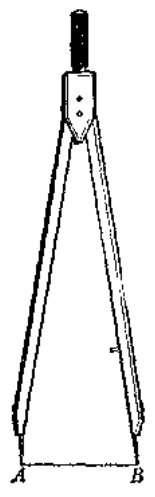
\includegraphics[width=2cm]{../pic/czjh1-ch1-13-a.png}
            \caption*{甲}
        \end{minipage}
        \qquad
        \begin{minipage}[b]{3cm}
            \centering
            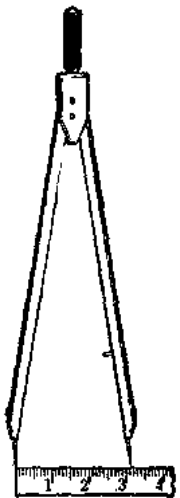
\includegraphics[width=2.3cm]{../pic/czjh1-ch1-13-b.png}
            \caption*{乙}
        \end{minipage}
        \caption{}\label{fig:czjh1-1-13}
    \end{minipage}
    \qquad
    \begin{minipage}[b]{7cm}
        \centering
        \begin{tikzpicture}[scale=1.5]
	\tkzDefPoints{0/0/A, 3/0/B, 2/0.8/C}
	\tkzDefMidPoint(A,B)  \tkzGetPoint{O}
	\tkzDrawPolygon(A,B,C)
	\tkzDrawArc(O,B)(A)
	\tkzLabelPoints[left](A)
	\tkzLabelPoints[right](B)
	\tkzLabelPoints[above](C)

	\tkzDefPoints{0.8/-0.4/a, 1.2/-0.2/b, 2.3/-0.8/c}
	\tkzDrawSegments(A,a a,b b,c c,B)
\end{tikzpicture}


        \caption{}\label{fig:czjh1-1-14}
    \end{minipage}
\end{figure}


把两点 $A$、$B$ 用线段和其他不同形状的线连结起来(图 \ref{fig:czjh1-1-14}),然后把这些线拉直,
进行比较,可以发现线段有下面的性质,我们把它作为公理:

\begin{gongli}[公理]\label{theorem:ldzjxdzd}
    在所有连结两点的线中,线段最短。
\end{gongli}

这句话可以简单地说成:\begin{gongli}
    两点之间线段最短。
\end{gongli}

连结两点的线段的长度,叫做\zhongdian{两点的距离。}


\begin{lianxi}

\xiaoti{用两脚规配合刻度尺量出图 \ref{fig:czjh1-1-14} 中线段 $AB$、$AC$、$CB$ 的长度(确到 1 mm),
    并根据量出的结果比较线段 $AB$ 的长度与线段 $AC$、$BC$ 的长度的和的大小。
}

\xiaoti{可以利用两脚规来比较两条线段,如图甲那样,先将两脚规的两个脚的针尖分别对准线段 $AB$ 的两个端点,
    然后把两脚规的针尖所代表的线段 $AB$ 放到线段 $CD$ 上,使一个针尖落在线段 $CD$ 的一个端点上,
    根据另一个针尖所落的位置就可以判断两线段之间的大小。
    利用这个办法比较图乙中三条线段的大小,再比较图丙中两条线段 $AB$、$CD$的大小。
}

\begin{figure}[htbp]
    \centering
    \begin{minipage}[b]{4cm}
        \centering
        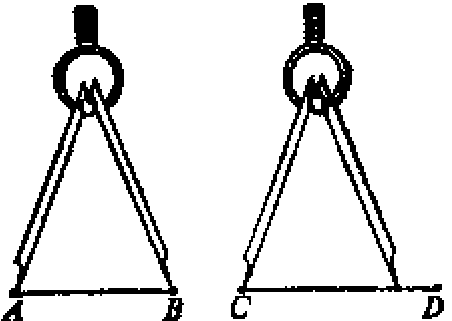
\includegraphics[width=3.8cm]{../pic/czjh1-ch1-subsec3-lx-2-a.png}
        \caption*{甲}
    \end{minipage}
    \qquad
    \begin{minipage}[b]{5cm}
        \centering
        \begin{tikzpicture}
	\tkzDefPoints{0/0/A, 3/0/B, 2/1.5/C}
	\tkzDrawPolygon(A,B,C)
	\tkzLabelPoints[left](A)
	\tkzLabelPoints[right](B)
	\tkzLabelPoints[above](C)
\end{tikzpicture}


        \caption*{乙}
    \end{minipage}
    \qquad
    \begin{minipage}[b]{4cm}
        \centering
        \begin{tikzpicture}[scale=0.7]
	\tkzDefPoints{0/0/A, 3/0/B, 2/0/C, 2/3/D}
	\tkzDrawSegments(A,B  C,D)
	\tkzLabelPoints[above](D)
	\tkzLabelPoints[below](A,B,C)
\end{tikzpicture}


        \caption*{丙}
    \end{minipage}
    \caption*{(第 2 题)}
\end{figure}

\xiaoti{用刻度尺度量出上题的图乙中各线段的长度; 丙中点 $A$、$D$, 点 $B$、$D$ 的距离。}

\end{lianxi}

